\subsection{3D Diamond Detectors}
\begin{frame}{Detector Concept}

	\vspace*{-5pt}
	\begin{itemize}
		\itemfill
		\item after large irradiation \ra all detector materials trap limited (mfp < \SI{75}{\micro\meter})
		\item \usebeamercolor[fg]{title} \textbf{keep drift distances smaller than mean free path}
	\end{itemize}

	\vspace*{-10pt}
	\begin{figure} 
		\begin{center}
			\begin{subfigure}{0.4\textwidth}  
				\centering 
				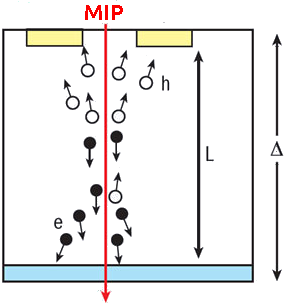
\includegraphics[height=.44\textheight]{PlanarConcept}
				\caption{planar detector}
			\end{subfigure}
			\begin{subfigure}{0.1\textwidth}  
				\centering 
				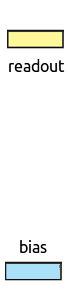
\includegraphics[height=.44\textheight]{LegendConcept}
				\vspace*{20pt}
			\end{subfigure}
			\begin{subfigure}{0.4\textwidth} 
				\centering 
				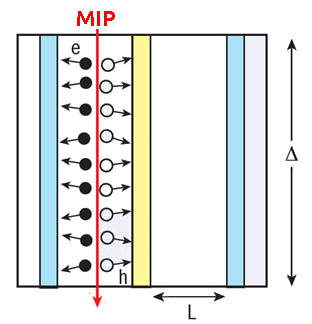
\includegraphics[height=.44\textheight]{3DConcept}
				\caption{3D detector} 	
			\end{subfigure} 
		\end{center}
	\end{figure}\vspace*{-15pt}
	
	\begin{itemize}
		\itemfill
		\item bias and readout electrode inside detector material
		\item same thickness $\Updelta$ \ra same amount of induced charge \ra shorter drift distance L
		\item electrode columns drilled with \SI{800}{\nano\meter} femtosecond laser 
		\item convert diamond into resistive mixture of carbon phases
	\end{itemize}

\end{frame}

% ============================ FRAME 2 ============================================
% \begin{frame}{3D Diamond Detectors}
% 
% 	\begin{itemize}
% 		\itemfill
% 		\item columns drilled with \SI{800}{\nano\meter} femtosecond laser 
% 		\item convert diamond into resistive mixture of carbon phases
% 	\end{itemize}
% 	
% 	\begin{figure}
% 		\centering 
% 		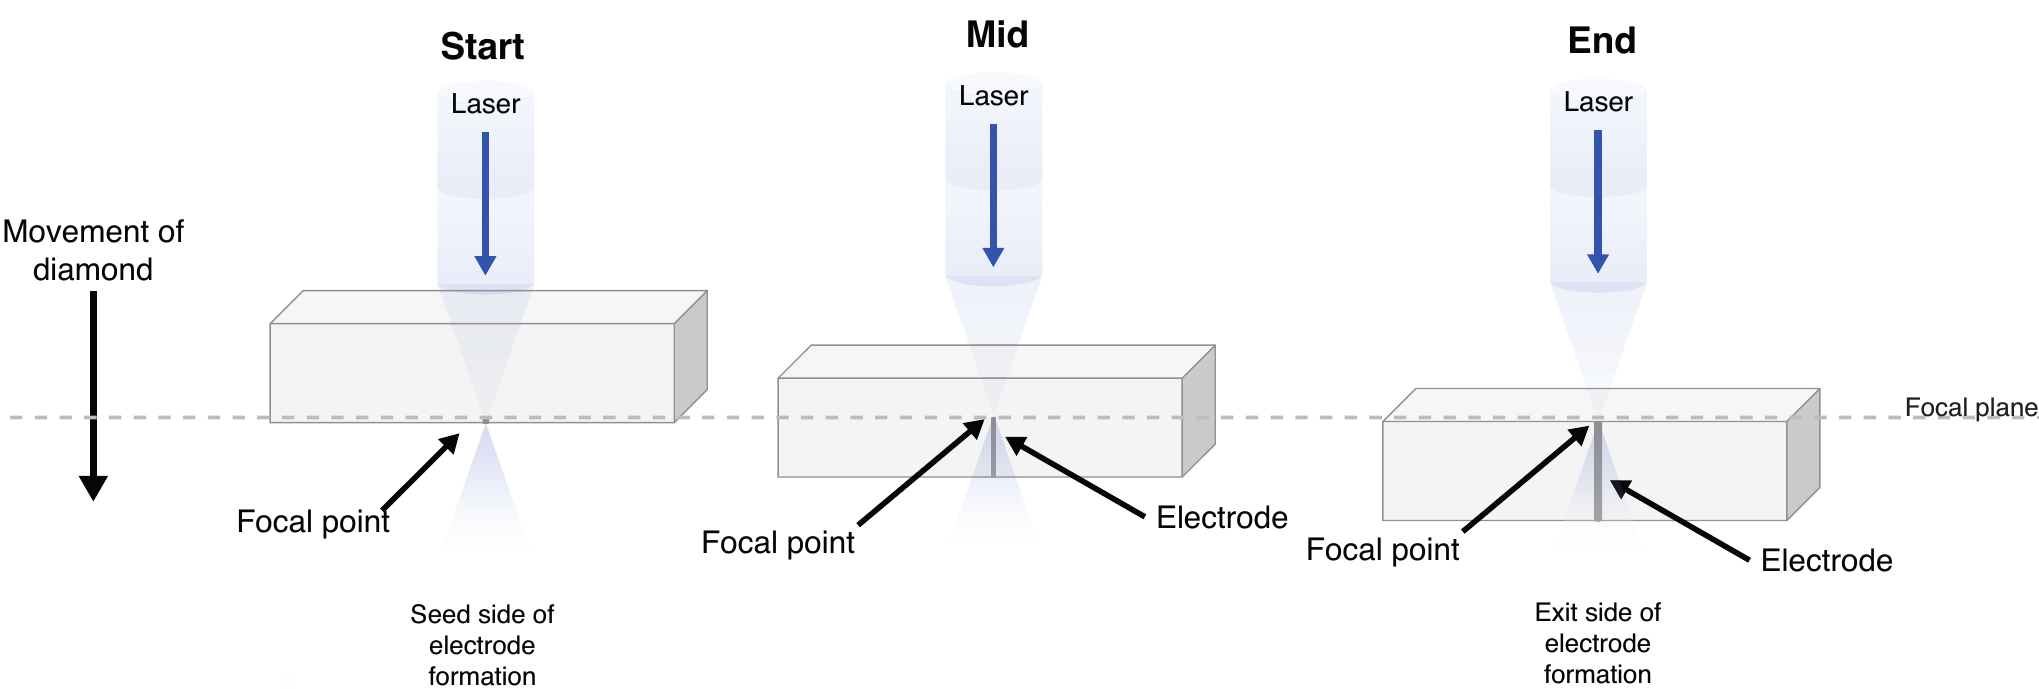
\includegraphics[width=.9\textwidth]{Fabrication}
% 	\end{figure}
% 	
% 	\begin{itemize}
% 		\itemfill
% 		\item 3 years ago: results of scCVD diamond detector
% 		\item 2 years ago: first 3D device in pCVD
% 		\item last year: first 3D pixel detector in pCVD diamond
% 	\end{itemize}
% 
% \end{frame}

% ============================ FRAME 3 ============================================
\begin{frame}{3D Multi Detector (2015)}

	\begin{itemize}
		\itemfill
		\item pCVD diamond with 3D, phantom and strip detector on single sensor
		\item 3D column efficiency of \SI{92}{\%}
		\item 3D cell size: \SI{150x150}{\micro\meter}
		\item signal read out as ganged cells
	\end{itemize}
	
	\begin{figure}
		\centering
		\begin{subfigure}{0.45\textwidth}  
			\centering 
			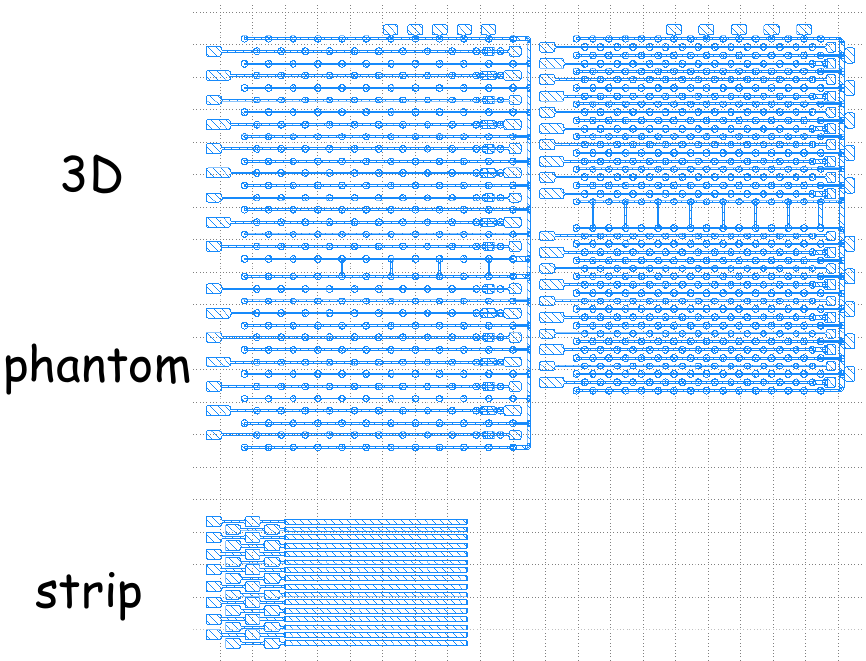
\includegraphics[height=.44\textheight]{3DMultiScheme}
			\caption{metalisation pattern}
		\end{subfigure}
		\begin{subfigure}{0.45\textwidth} 
			\centering 
			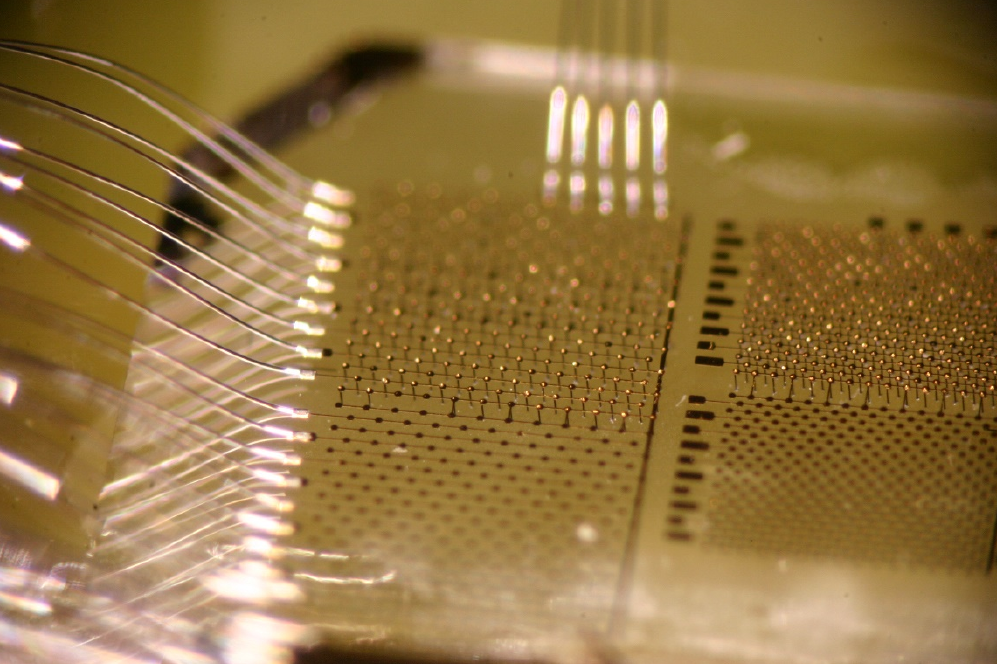
\includegraphics[height=.44\textheight]{3DMulti2}
			\caption{photograph}
		\end{subfigure}
	\end{figure}\vspace*{-15pt}

\end{frame}

% ============================ FRAME 4 ============================================
\begin{frame}{3D Multi - Signal Map}

	\begin{itemize}
		\itemfill
		\item square cells visible (9 broken cells)
		\item signals in 3D already bigger by eye
		\item phantom (no columns) \ra no pulse height
	\end{itemize}
	
	\begin{figure}
		\centering 
		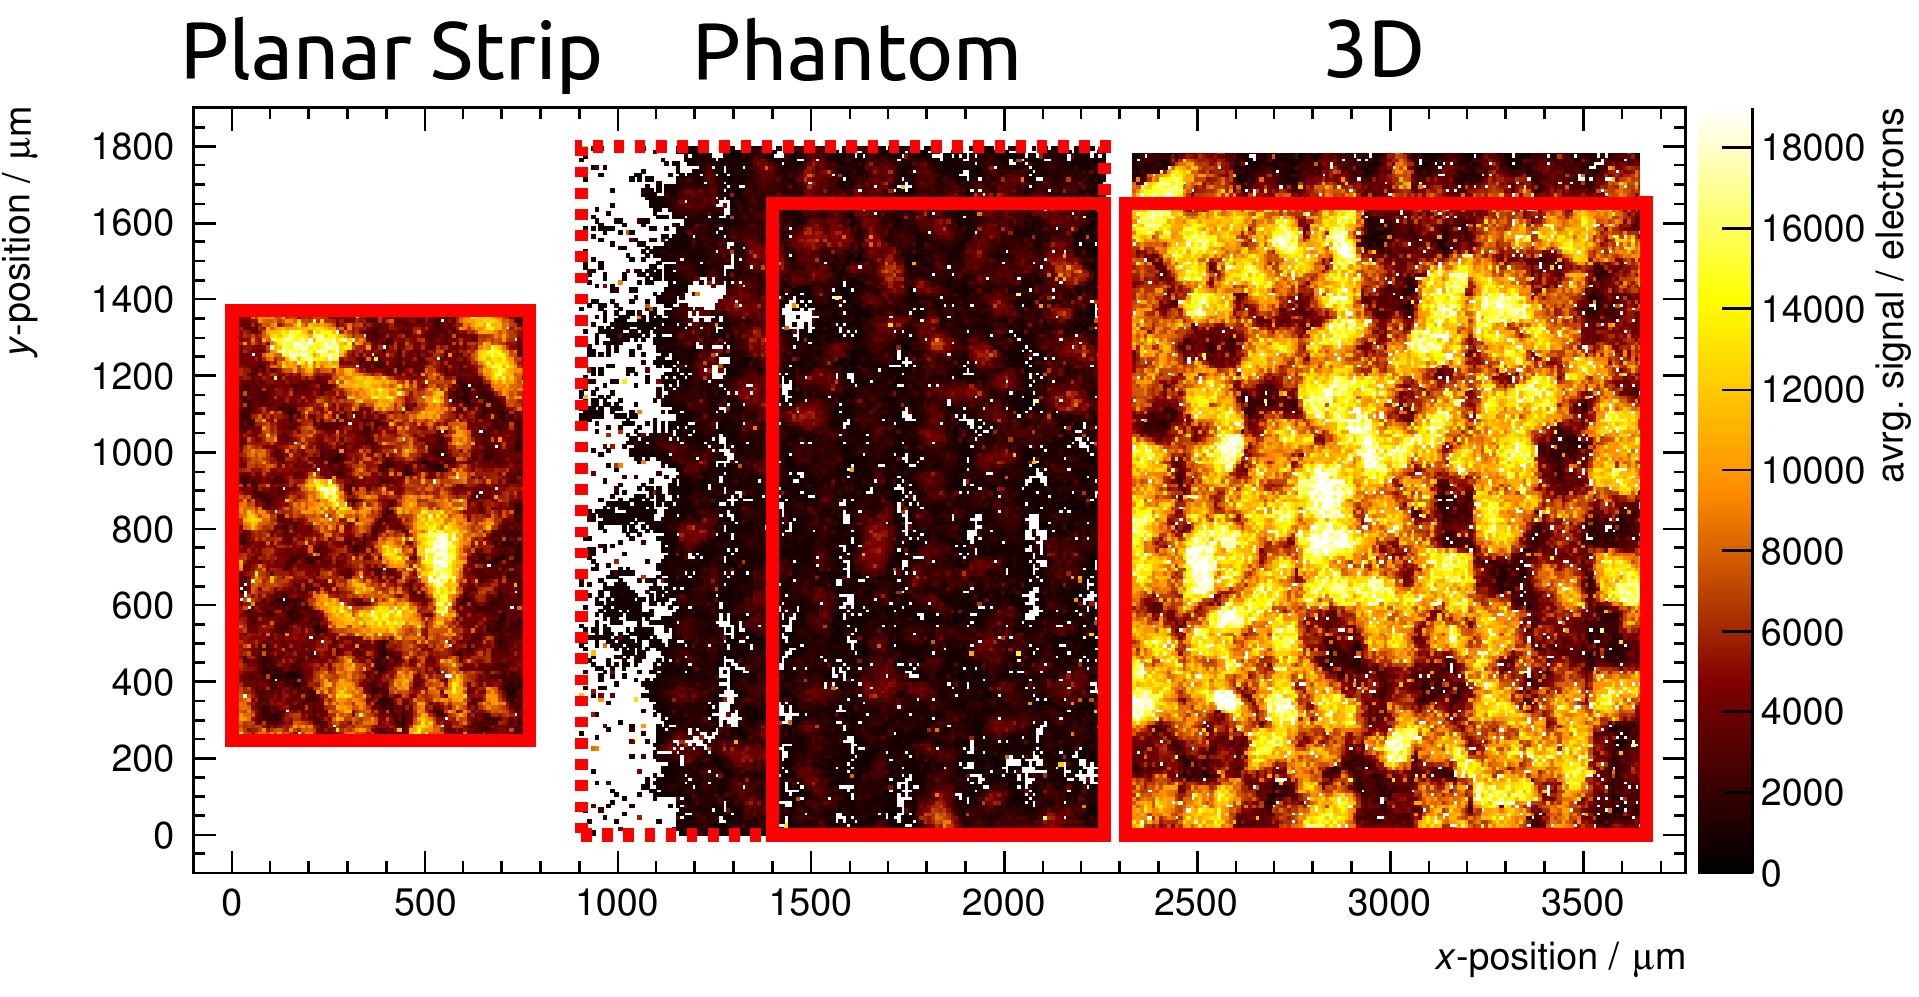
\includegraphics[height=.6\textheight]{3DMulti1}
	\end{figure}\vspace*{-10pt}

\end{frame}
% ============================ FRAME 5 ============================================
\begin{frame}{3D Multi - Result}

	\begin{itemize}
		\itemfill
		\item measured signals for diamond thickness \SI{500}{\micro\meter}:
	\end{itemize}
	
	\begin{table}
		\begin{tabular}[c]{c|c|c}
			\noalign{\hrule height 1pt}
			\rowcolor{title in head/foot.bg!70!white} 
			\multicolumn{1}{c|}{\textbf{Device}} & \multicolumn{1}{c|}{\textbf{Mean Charge [e]}} & \multicolumn{1}{c}{\textbf{ccd [$\upmu$m]}} \\\hline
			\rowcolor{date in head/foot.bg!30!white} 
			planar strip 	& $6900$ 	& $192$ 		\\\hline
			3D				& $13500$ 	& $350 - 375$* 	\\\hline
			\noalign{\hrule height 1pt}
		\end{tabular}
	\end{table}
	\begin{itemize}
		\itemfill
		\item *ccd$_{\z{eq}}$ - equivalent ccd to observe same charge in planar device
		\item \good{collect > \SI{75}{\%} charge in pCVD for the first time}
	\end{itemize}
	
	\begin{figure}
		\centering 
		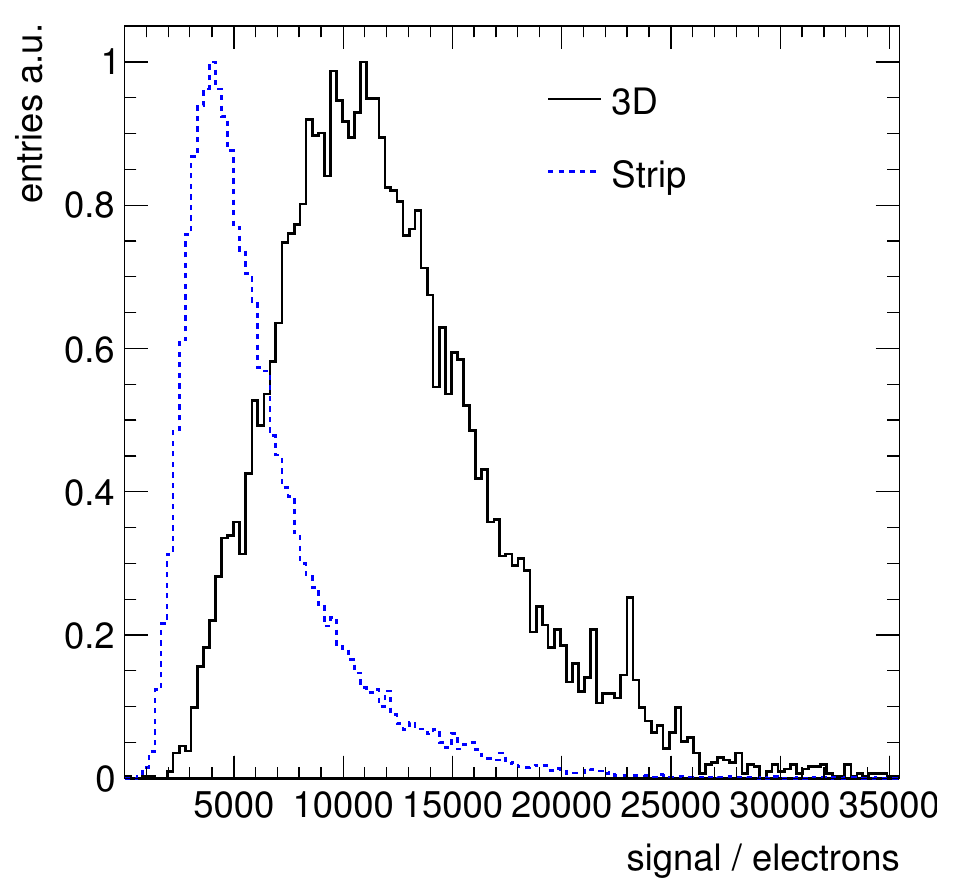
\includegraphics[height=.5\textheight]{3DMultiResult}
	\end{figure}\vspace*{-10pt}

\end{frame}
% ============================ FRAME 6 ============================================
\begin{frame}{Full 3D Detector (May/Sep 2016)}

	\begin{itemize}
		\itemfill
		\item 3 dramatic improvements compared to 3D Multi:
		\vspace*{3pt}
			\begin{itemize}
				\itemfill
				\item an order of magnitude more cells: from \SIrange{99}{1188}{}
				\item smaller cell size: \SI{100x100}{\micro\meter}
				\item higher column efficiency: from \SIrange{92}{99}{\%}
			\end{itemize}

	\end{itemize}
	
	\begin{figure}
		\centering
		\begin{subfigure}{0.45\textwidth}  
			\centering 
			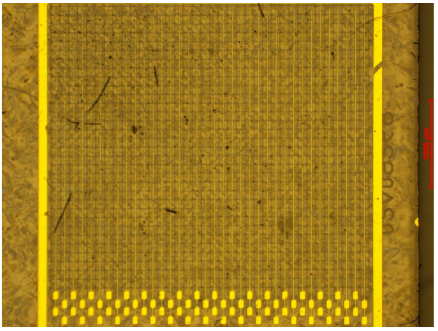
\includegraphics[height=.48\textheight]{3DFull1}
			\caption{readout side}
		\end{subfigure}
		\begin{subfigure}{0.45\textwidth} 
			\centering 
			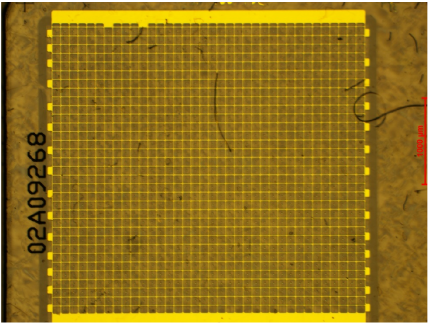
\includegraphics[height=.48\textheight]{3DFull2}
			\caption{bias side}
		\end{subfigure}
	\end{figure}\vspace*{-15pt}

\end{frame}
% ============================ FRAME 6 ============================================
\begin{frame}{Full 3D Preliminary Results}

	\begin{itemize}
		\itemfill
		\item analysis in progress
		\item device seems to perform well
		\item see charge in entire detector
		\item largest charge collection in pCVD yet
		\begin{itemize}
			\vspace*{1pt}
			\item \good{\SI{>85}{\%} over contiguous region}
		\end{itemize}
	\end{itemize}
	
	\vspace*{-5pt}
	\begin{figure}
		\centering
		\begin{subfigure}{0.45\textwidth}  
			\centering 
			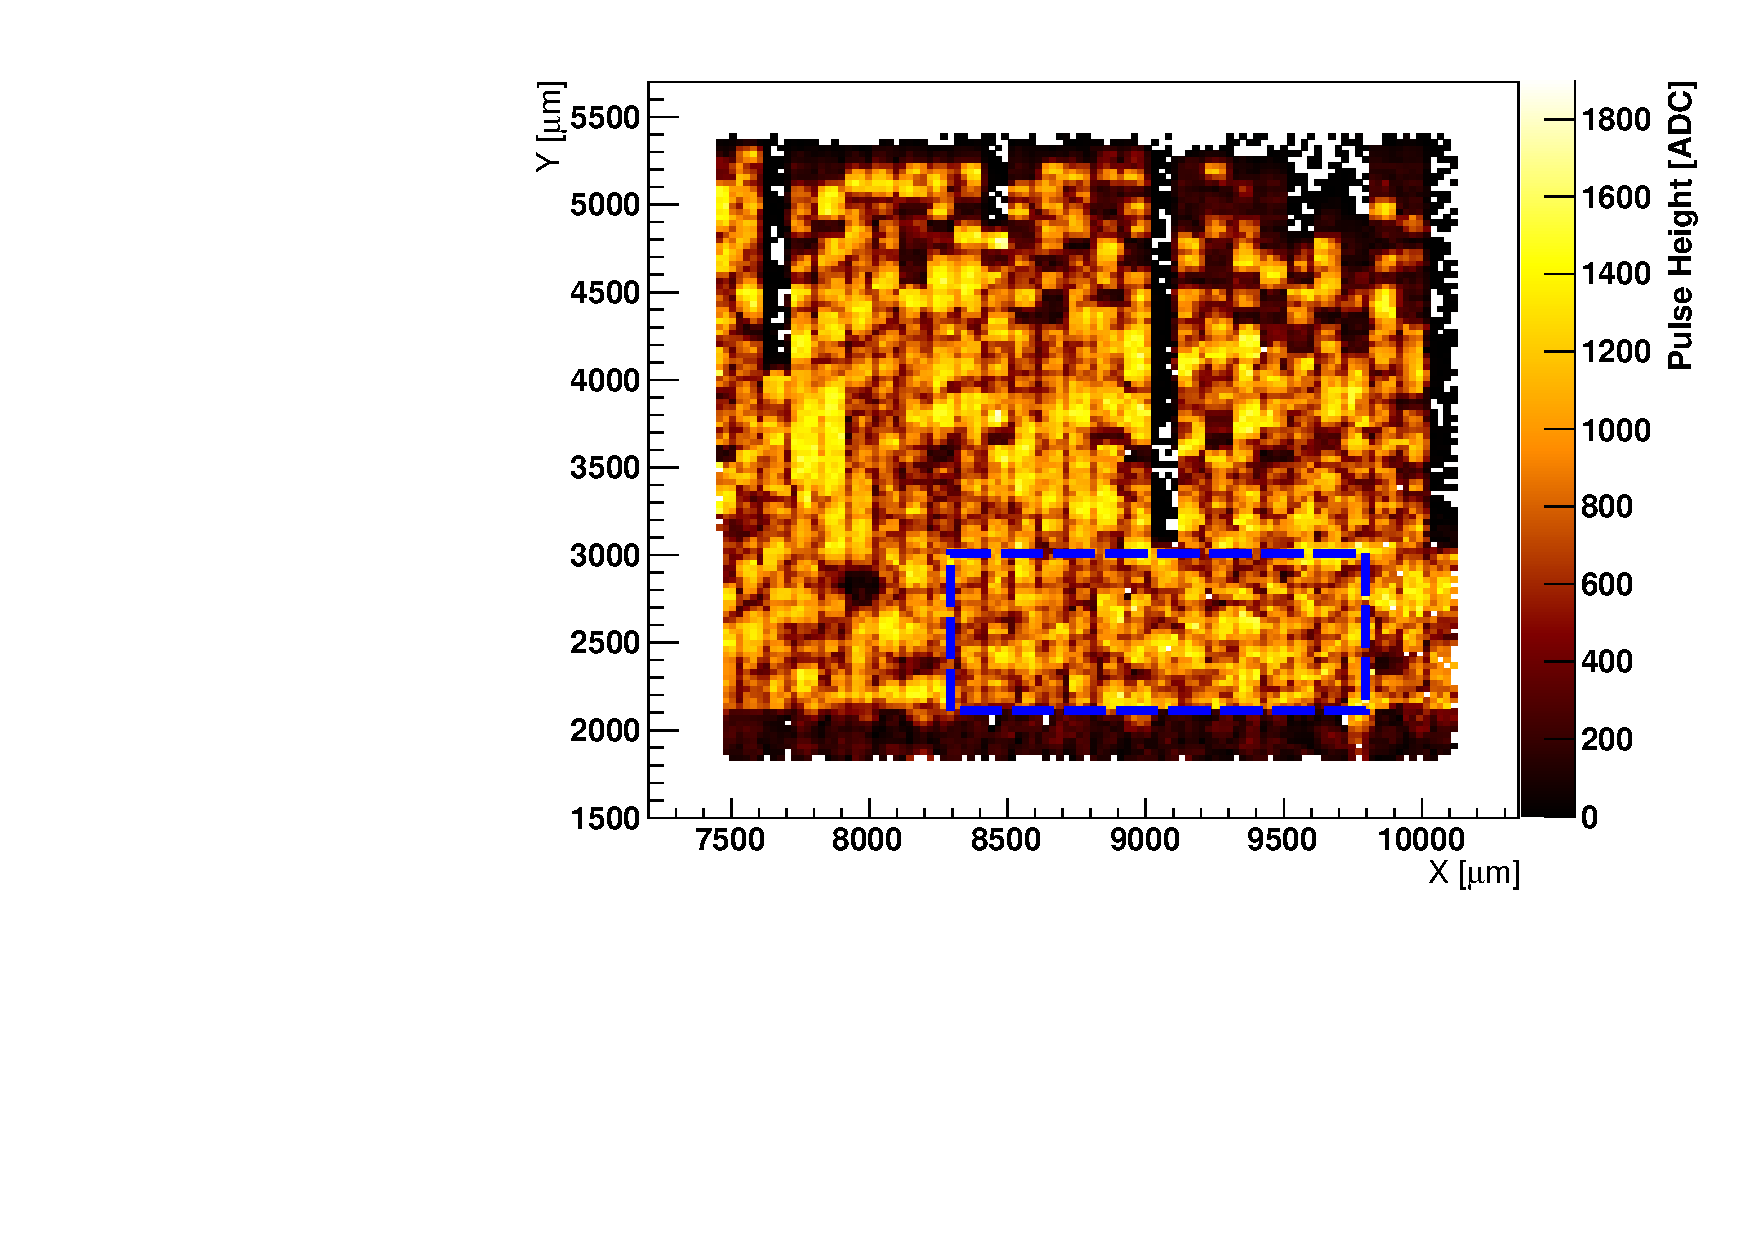
\includegraphics[width=.5\textheight, angle=-90]{3DFullCharge}
			\caption{charge map}
		\end{subfigure}
		\begin{subfigure}{0.45\textwidth} 
			\centering 
			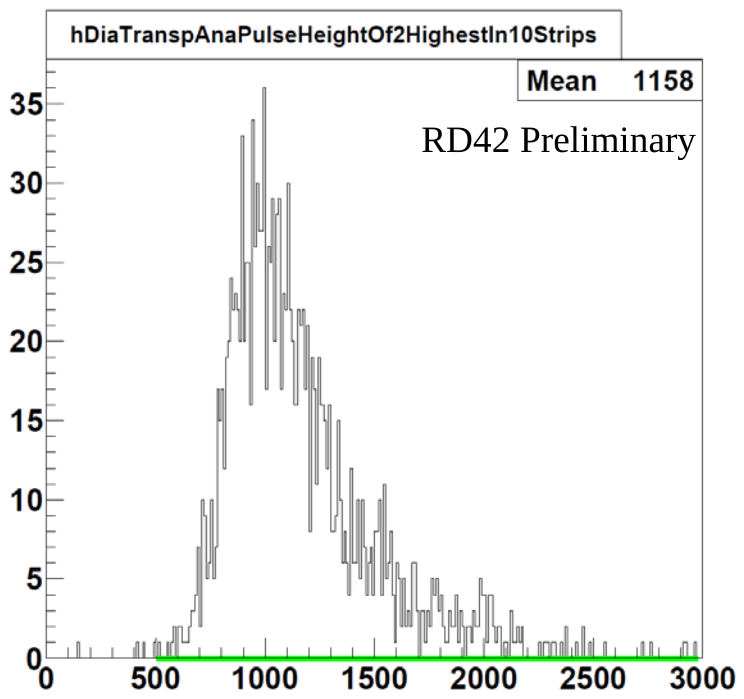
\includegraphics[width=.5\textheight, angle=-90]{3DFullDisto}
			\caption{charge distribution}
		\end{subfigure}
	\end{figure}\vspace*{-15pt}

\end{frame}

% ============================ FRAME 7 ============================================
\begin{frame}{3D Pixel Detector - Fabrication}

	\vspace*{-5pt}
	\begin{itemize}
		\itemfill
		\item cleaning and photo-lithography
		\item connect to bias and readout with surface metallisation
		\item bump and wire bonding
	\end{itemize}
	
	\begin{figure}
		\centering
		\begin{subfigure}{0.45\textwidth}  
			\centering 
			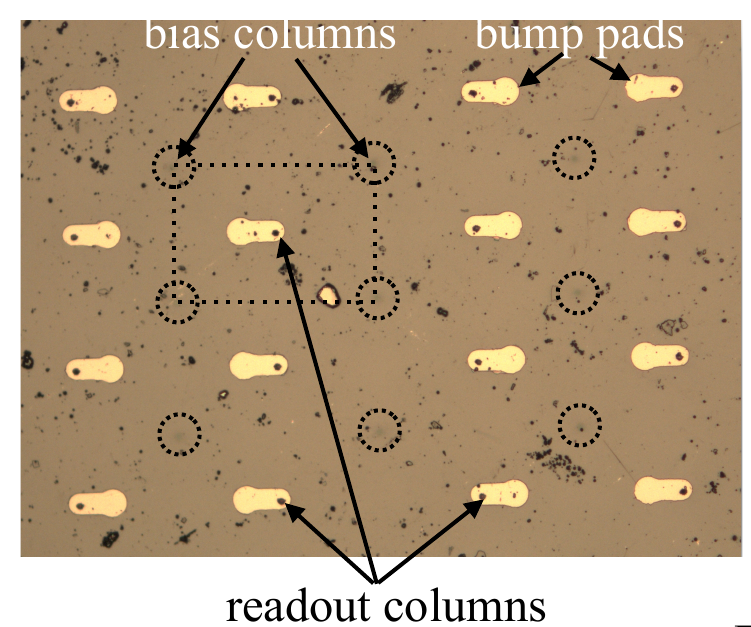
\includegraphics[height=.48\textheight]{BumpPads}
			\caption{pixel readout metalisation}
		\end{subfigure}
		\hspace*{10pt}
		\begin{subfigure}{0.45\textwidth} 
			\centering 
			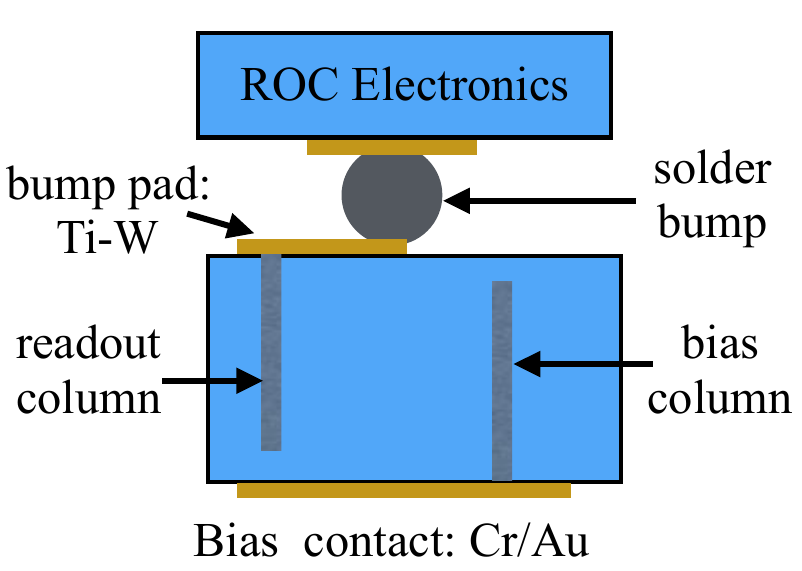
\includegraphics[height=.48\textheight]{FabFinalScheme}
			\caption{final scheme}
		\end{subfigure}
	\end{figure}\vspace*{-15pt}
 	
\end{frame}
% ============================ FRAME 7 ============================================
\begin{frame}{3D Pixel Detector}
	
	\begin{figure}
		\centering
		\begin{subfigure}{0.45\textwidth}  
			\centering 
			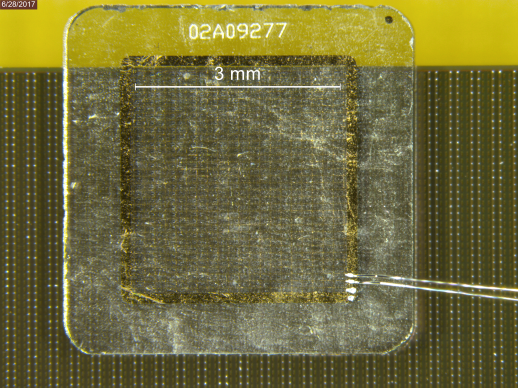
\includegraphics[height=.44\textheight]{3DFull}
			\caption{detector bonded on CMS-Pixel-Chip}
		\end{subfigure}
		\begin{subfigure}{0.45\textwidth} 
			\centering 
			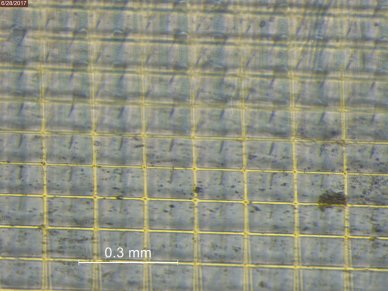
\includegraphics[height=.44\textheight]{3DCols}
			\caption{bias grid and R/O columns}
		\end{subfigure}
	\end{figure}

	\begin{itemize}
		\itemfill
		\item successful production of a working 3D pixel detector
	\end{itemize}
 	
\end{frame}
% ============================ FRAME 8 ============================================
\begin{frame}{3D Pixel Detector - Preliminary Results}

	\begin{minipage}{.4\textwidth}
		\hfill 3D Diamond Pixel\\
		\good{\hfill\ra\SI{98.5}{\%} Efficiency}
		
		\vspace*{20pt}
		\color{black}
		\begin{itemize}
			\color{black}
			\item efficiencies flat in time
			\item pixel threshold: \SI{1500}{e}
			\item lower efficiency in diamond probably due to due to low field regions
		\end{itemize}
		\vspace*{20pt}
		
		\hfill Planar Silicon Pixel (Ref)\\
		\good{\hfill\ra\SI{99.3}{\%} Efficiency}

	\end{minipage}
	\hspace*{2pt}
	\begin{minipage}{.56\textwidth}
		\begin{figure}[h]
			\centering
			\begin{subfigure}{0.45\textwidth}  
				\centering 
				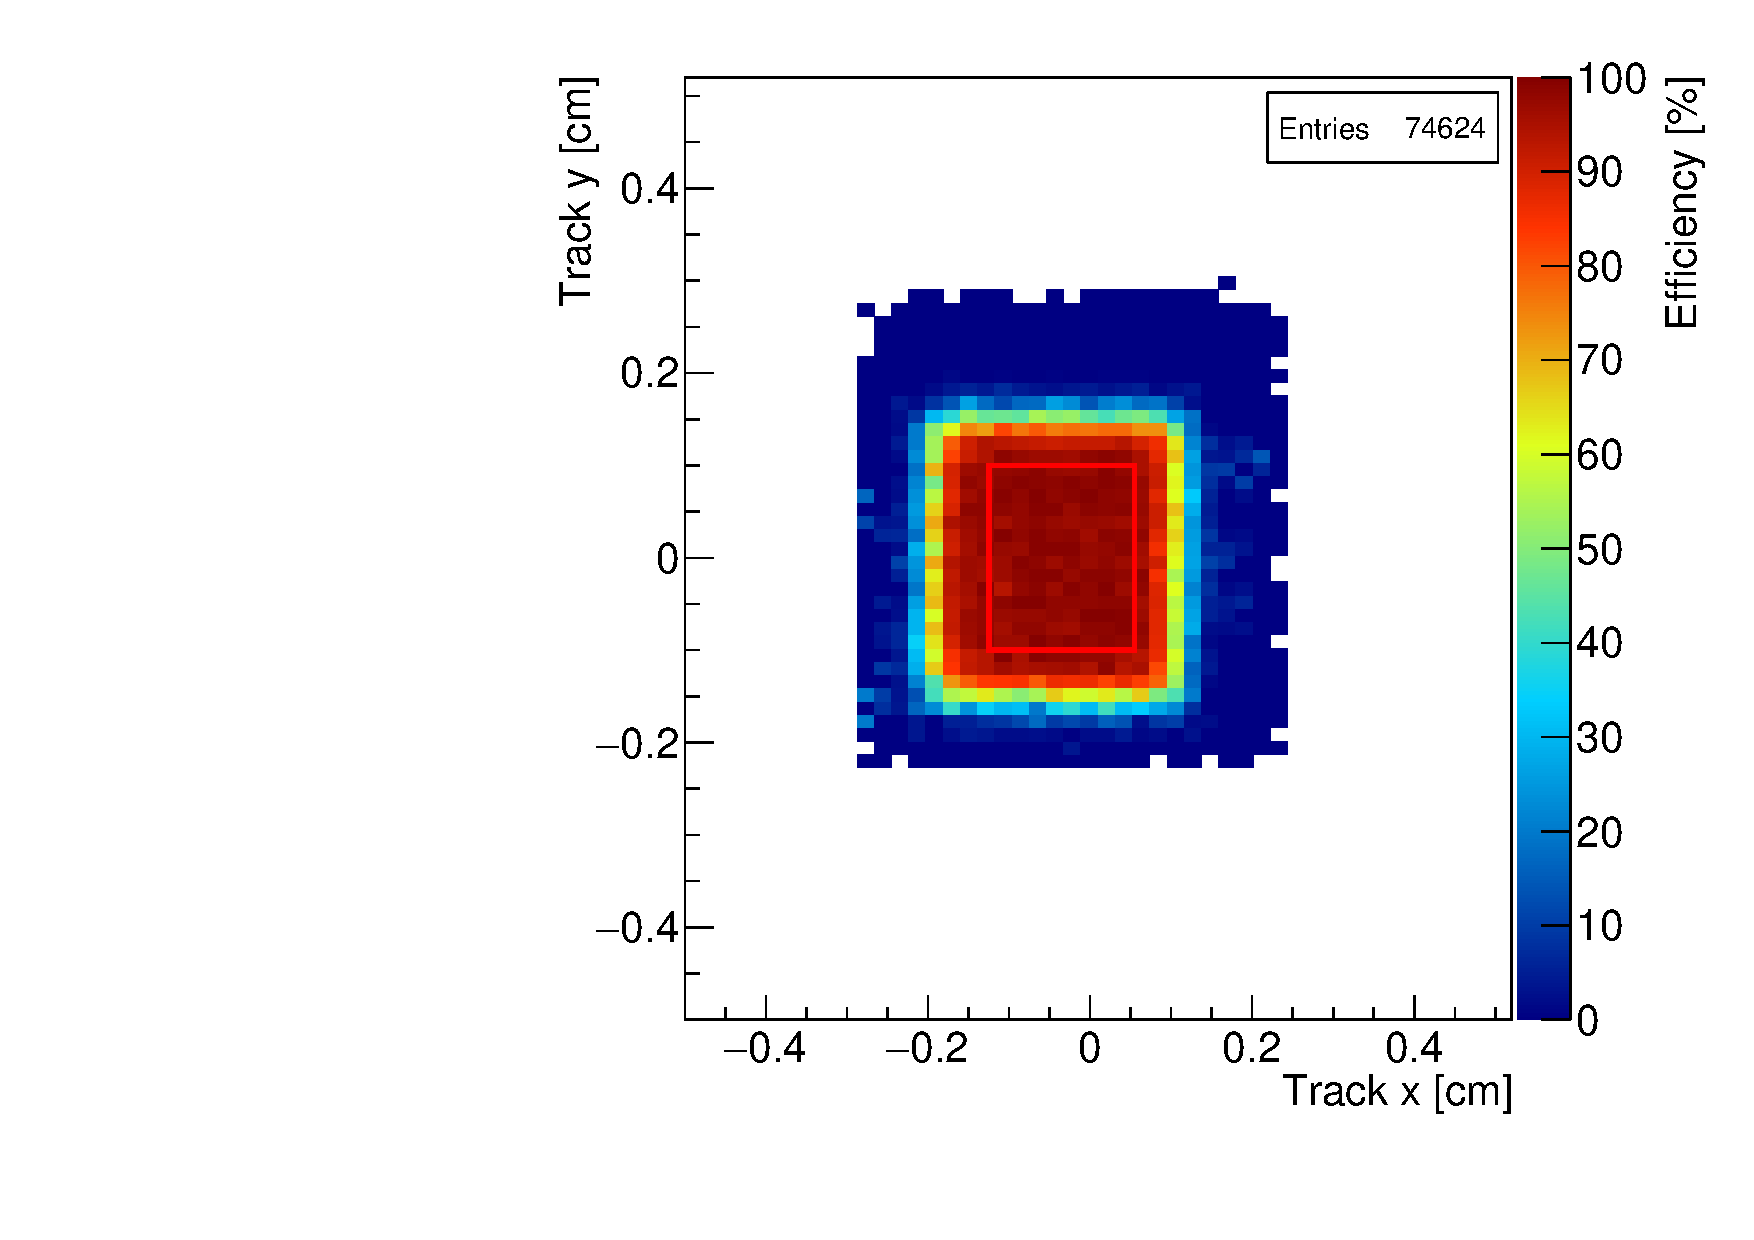
\includegraphics[width=.4\textheight, angle=-90]{EffMapDia}
			\end{subfigure}
			\begin{subfigure}{0.45\textwidth} 
				\centering 
				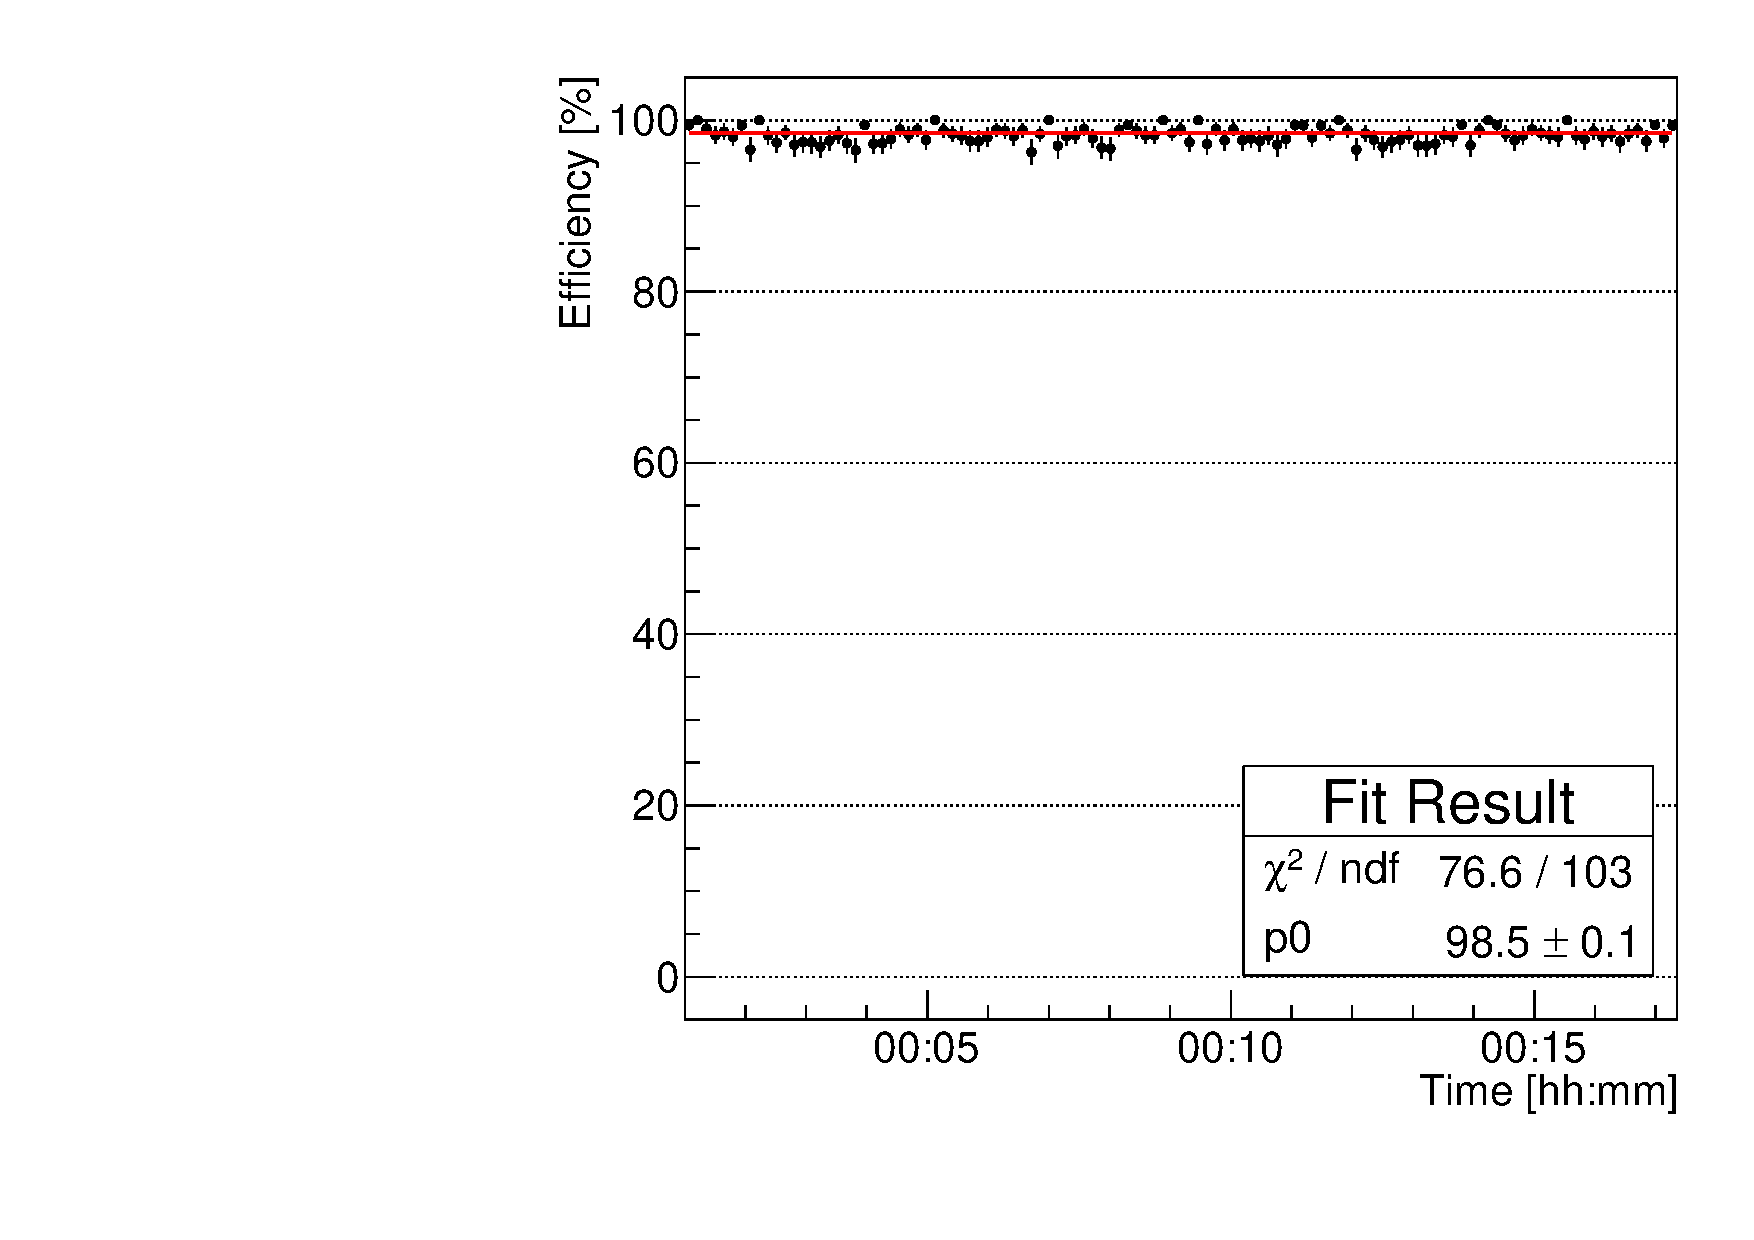
\includegraphics[width=.4\textheight, angle=-90]{HitEffDia}
			\end{subfigure}
			\begin{subfigure}{0.45\textwidth}  
				\centering 
				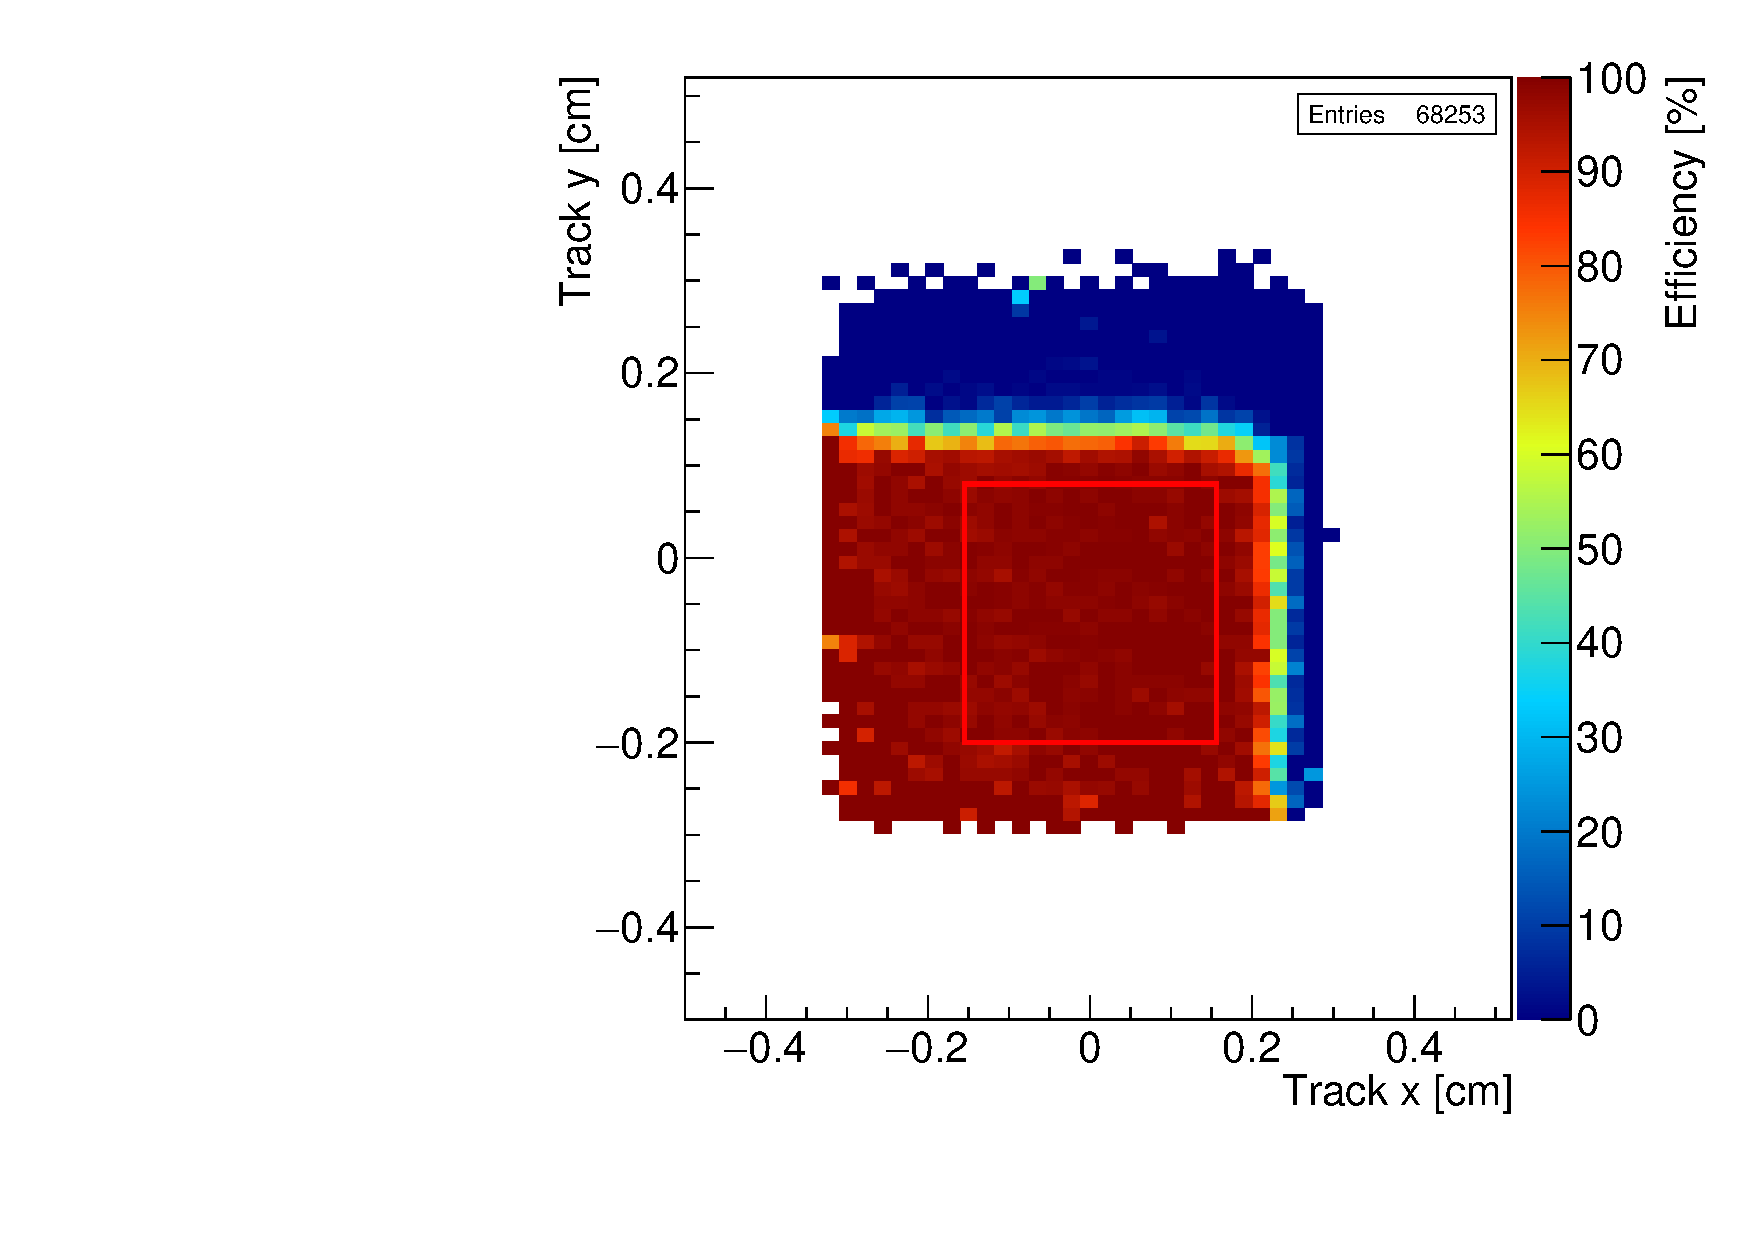
\includegraphics[width=.4\textheight, angle=-90]{EffMapSil}
				\caption{efficiency maps}
			\end{subfigure}
			\begin{subfigure}{0.45\textwidth} 
				\centering 
				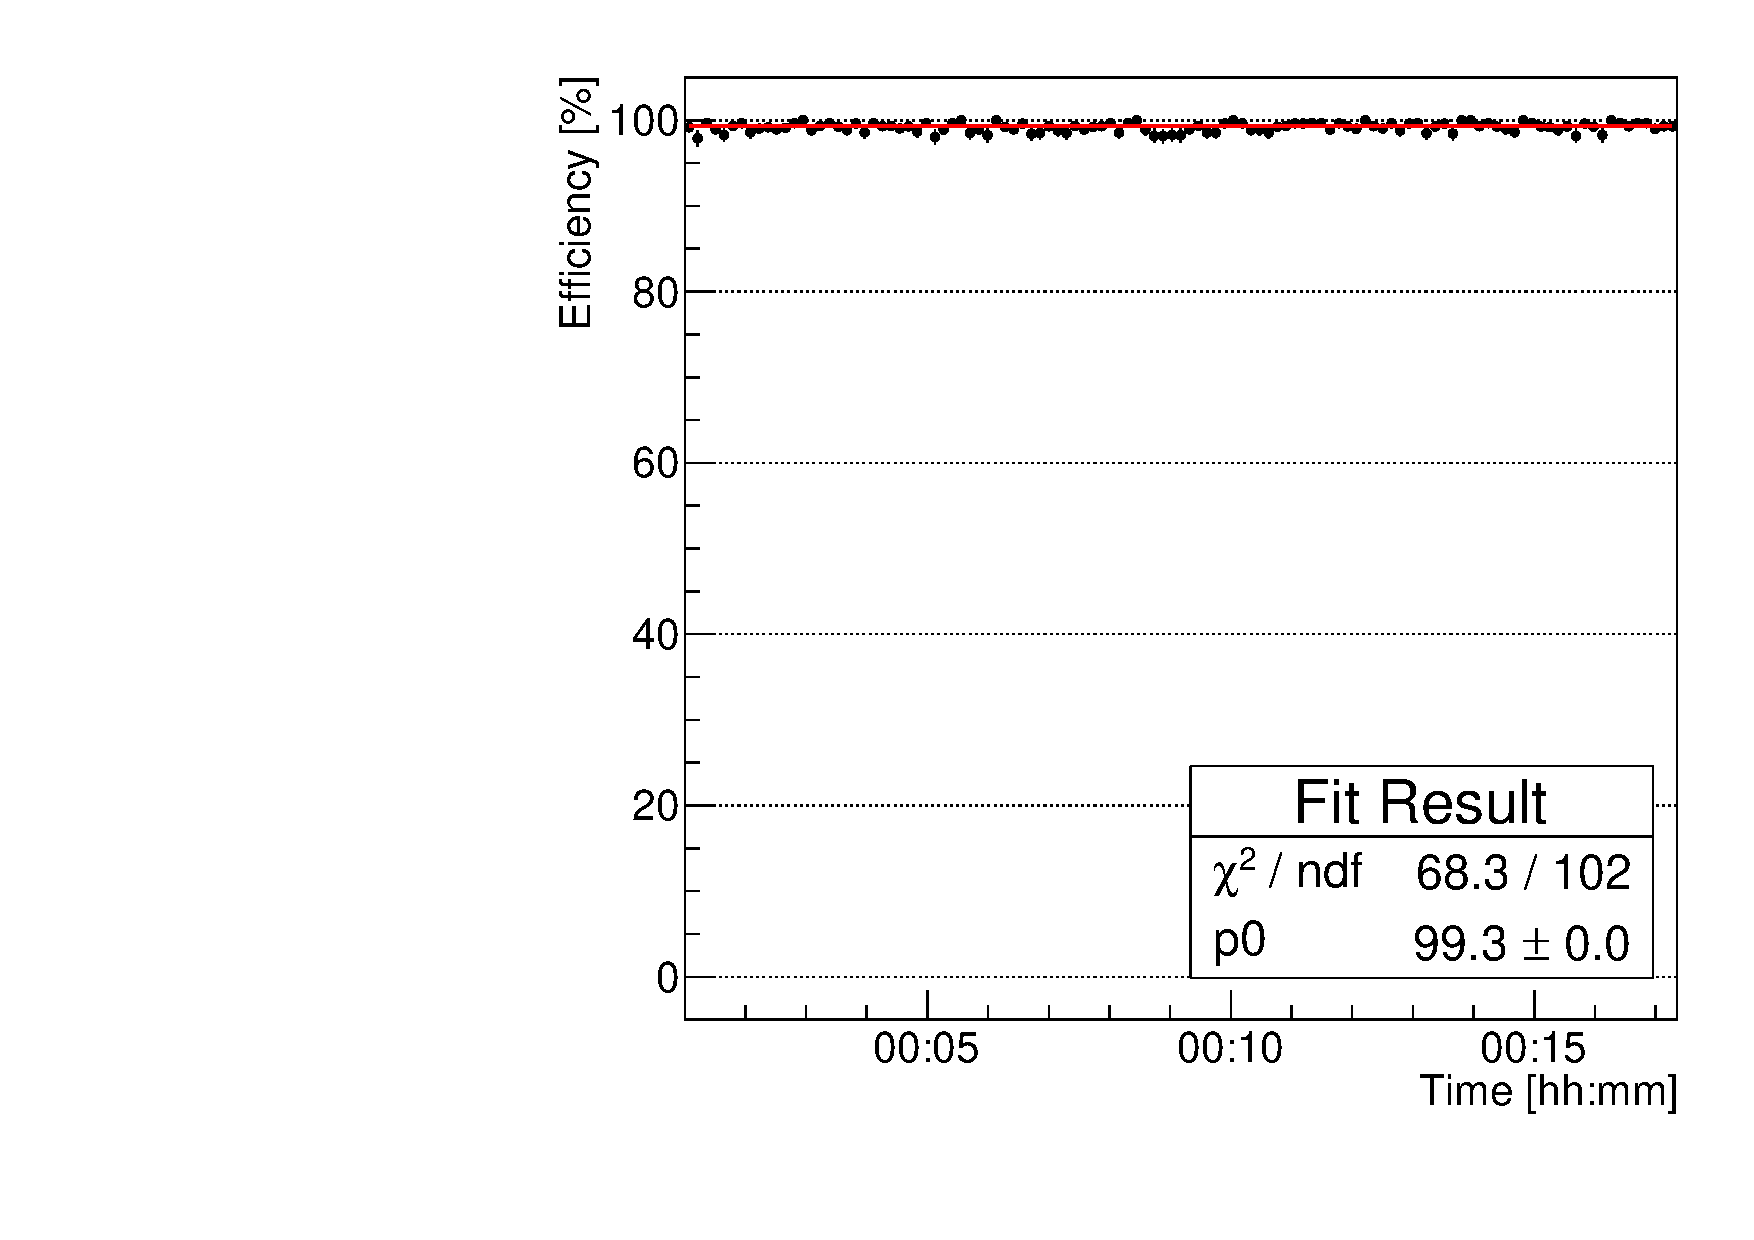
\includegraphics[width=.4\textheight, angle=-90]{HitEffSil}
				\caption{hit efficiencies}
			\end{subfigure}
		\end{figure}
	\end{minipage}
 	
\end{frame}
% ============================ FRAME 9 ============================================
\begin{frame}{3D Pixel Detector - New Design}

	\vspace*{-5pt}
	\begin{itemize}
		\itemfill
		\item currently producing \SI{3500}{cell} pixel prototype with \SI{50}{\micro\meter} pixel pitch
		\item two independent drillings (Oxford - complete, Manchester - in progress)
		\item bump bonding at Princeton (CMS) and IFAE (ATLAS)
		\item CMS device probably ready for August beam tests
	\end{itemize}\vspace*{-10pt}
	
	\begin{figure}
		\centering 
		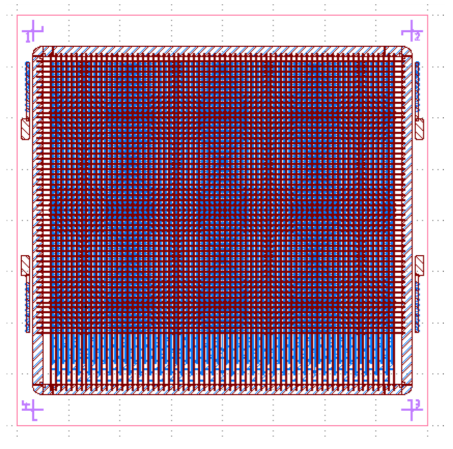
\includegraphics[height=.6\textheight]{3DNew}
	\end{figure}\vspace*{-15pt}
 	
\end{frame}

